\documentclass{article}
\usepackage{graphicx} % Required for inserting images
\usepackage[labelformat=empty]{caption}
\usepackage{hyperref}
\usepackage[top=1.0in, bottom=1.0in]{geometry}
\usepackage{enumitem}
\graphicspath{ {./images/} }
\date{}

\title{CS 699 - Project\\ Bird Image Classification and Visualization}


\begin{document}

\maketitle

\section{Image Classification}

\noindent Uploaded image:

\begin{figure}[h!]
\centering
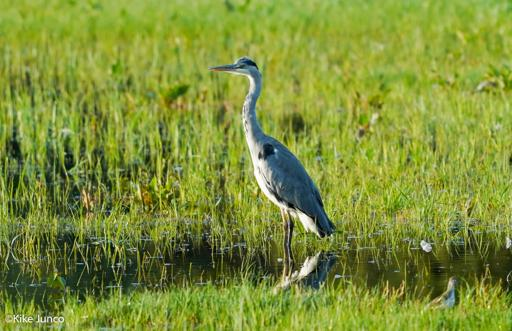
\includegraphics[width=100mm]{/Users/smitjivani/Developer/MS_WS/CS699/Project/CS699_Project/report/images/bird_test.jpg}
\caption*{Prediction: Grey Heron}
\label{fig:method}
\end{figure}

\noindent Classifier: SVM
\newline
\newline
\newline
\noindent Top 5 predictions:
\newline
\begin{table}[h!]
\centering
\begin{tabular}{|c|c|c|} 
\hline
 S.No. & Species Name & Prediction Probability\\ 
\hline
 1 & Blue Jay & 0.27 \\ 
 \hline
 2 & Grey Heron & 0.26 \\  
 \hline
 3 & Indian Peafowl & 0.26 \\    
 \hline
 4 & Little Egret & 0.10 \\    
 \hline
 5 & Red-Vented Bulbul & 0.11 \\    
 \hline
\end{tabular}
\caption{Species wise prediciton probability}
\label{table:data}
\end{table}




\newpage
\section{Model Report}

\textbf{Classifier:} SVM
\newline

\noindent \textbf{Dataset:}
Images scrapped from \href{https://ebird.org/explore}{eBird Portal}  for species classification across 5 species.
\newline
Total images: 5000
\newline
Train-Test Split: 80:20
\newline
\newline
\noindent \textbf{Species:}
\begin{enumerate}[noitemsep]
  \item Blue Jay
  \item Grey Heron
  \item Indian Peafowl
  \item Little Egret
  \item Red-Vented Bulbul
\end{enumerate}
\vspace{5mm}
\noindent \textbf{Metrics:}
\newline
\newline
\noindent \textbf{Classification Report:}

\begin{verbatim}                   precision    recall  f1-score   support

         Blue Jay       0.30      0.25      0.27        12
       Grey Heron       0.27      0.50      0.35        12
   Indian Peafowl       0.56      0.42      0.48        12
     Little Egret       0.80      0.67      0.73        12
Red-Vented Bulbul       0.44      0.33      0.38        12

         accuracy                           0.43        60
        macro avg       0.47      0.43      0.44        60
     weighted avg       0.47      0.43      0.44        60
\end{verbatim}
\newpage
\noindent \textbf{Confusion Matrix:}

\begin{figure}[h!]
\centering
\includegraphics[width=100mm]{models/trained_models/SVM/conf.jpg}
\end{figure}
\noindent \textbf{Accuracy Plot:}
\begin{figure}[h!]
\centering
\includegraphics[width=100mm]{models/trained_models/SVM/accuracy.png}
\end{figure}
\end{document}
